\chapter{Introdu��o}
\label{cap:cap01}


\section{Se��o}
\label{sec:sec01}



Refer�ncia cita assim \cite{Cover2006}, \cite{Feynman1998,Haykin1998}, \cite{Cover2006,Feynman1998}.

Exemplo de uma f�rmula

\begin{equation}
H(X) =-K\sum_{x\in\mathcal{X}} p_X(x)\log p_X(x),
\label{eq:shannonEntropy1}
\end{equation}

A equa\c{c}\~{a}o pode ser citada assim~\eqref{eq:shannonEntropy1}, e a se\c{c}\~{a}o assim~\ref{sec:sec01}



Exemplo de uma figura.

\begin{figure}[htb]
\centering
	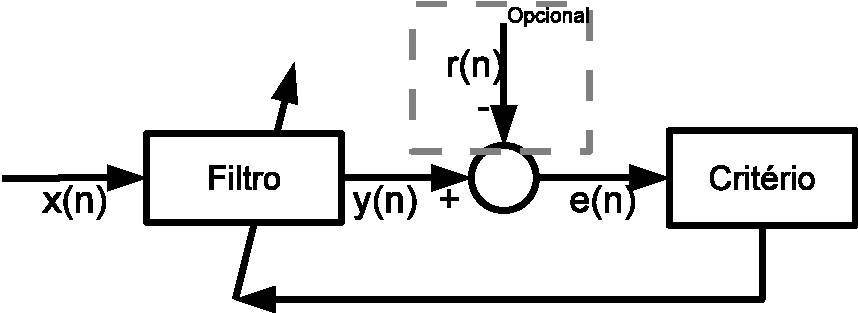
\includegraphics[width=.7\columnwidth]{./figs/filtering.pdf}
\caption{Esquema geral do problema de filtragem.}
\label{fig:filtering}
\end{figure}

\subsection{Subse��o}
\label{sec:subsec01}



Exemplo de lista.
\begin{itemize}
	\item bla bla bla 
	\item bla bla bla
\end{itemize}


Para mais informa��es sobre o Latex veja \href{http://tobi.oetiker.ch/lshort/lshort.pdf}{http://tobi.oetiker.ch/lshort/lshort.pdf}

\clearpage

Exemplo de Tabela

\begin{table}[ht]
\caption{Legenda da Tabela 1}
\begin{center}
\begin{tabular}{|c|c|c|}
\hline
\hline
\textbf{V} (m/s) & $\alpha$ (cm$^{-1}$) & $R$ (m) \\
3 & 34 & 23 \\
2 & 32 & 21 \\
\hline
\end{tabular}
\end{center}
\label{tab1}
\end{table}%
